 \documentclass[a4paper,10pt]{article}
\input{/Users/WannaGetHigh/workspace/latex/macros.tex}

\title{TI : TD sur la projection perspective}
\author{Fran�ois \bsc{Lepan}}

\begin{document}
\maketitle

\section{Images de droites et de plans}
\subsection{Quelle est l'�quation, dans le rep�re image, de la ligne d'horizon ?}
$l = T_y / 2$
\subsection{D�terminer les images}
\subsubsection{d'une droite verticale de vecteur directeur $\vec k$ passant par le point $(0, 10.f, 0)$ (20x , 30 x f aurai �t� pareil) }
une droite verticale passant par c \\
$c = T_x / 2$

\subsubsection{d'une droite horizontale de vecteur directeur $\vec i$ passant par le point $(0, 10.f, T_y)$ }
Une droite horizontale \\
on obtient avec les triangle semblable : (voir figure 1)\\

$[f, ?] = [ 10f, T_y ]$
$l = T_y/2 + T_y/ 10 = 2/5T_y$
$c = T_x/2$
\subsubsection{d'une demi-droite issue du point $(T_x, 10.f, T_y)$ dans la direction $\vec j$ ; }
$T_x / 10$ et a $T_y / 10$
$l =  T_y/2 + T_y/ 10 = 2/5T_y$

\begin{figure}[ht]
\begin{center}
     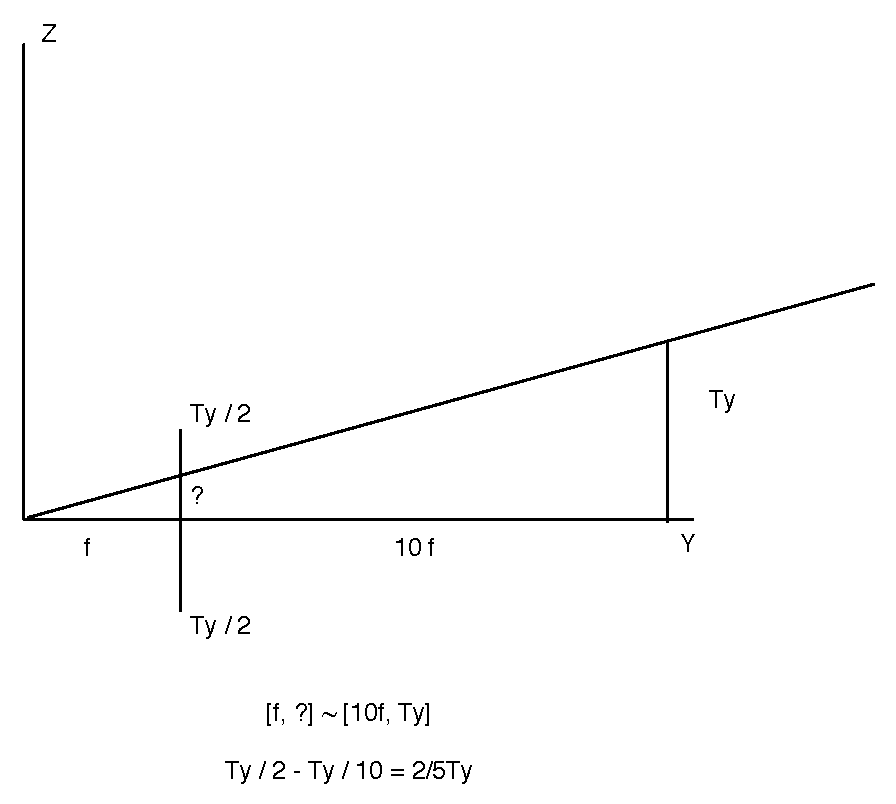
\includegraphics[width=15cm]{triangle_semblable.pdf}
\end{center}
     \caption{}
\end{figure}

\end{document}